\documentclass[xcolor=pdftex,dvipsnames,table,aspectratio=169]{beamer}
%\documentclass[xcolor=pdftex,dvipsnames,table,handout,aspectratio=169]{beamer}

%\setbeameroption{show notes}

\usepackage{bm,graphicx,multirow,amsmath,tikz} %fancybox,
\usepackage{color}%,textpos}
\usepackage[round]{natbib}
\usepackage[normalem]{ulem}
\usepackage{hyperref}
\usepackage{lastpage}
\usepackage{array}
\usepackage{color}
\usepackage{framed}
\usepackage{hyperref}

% Define Western colours
\definecolor{western}{rgb}{.306,.152,.524}
\definecolor{westerngray}{rgb}{.512,.508,.524}

%% Define BEAMER colours
\setbeamercolor{frametitle}{bg=western,fg=white}
\setbeamercolor{framesubtitle}{bg=western,fg=black}
\setbeamercolor{title}{fg=white,bg=western}
\setbeamercolor{author}{fg=white,bg=western}
\setbeamercolor{institute}{fg=white,bg=western}
\setbeamercolor{date}{fg=white,bg=western}

%% Set BEAMER fonts
\setbeamerfont{title}{shape=\bf}
\setbeamerfont{frametitle}{shape=\sc,size=\Large}
\setbeamerfont{framesubtitle}{shape=\sc,size=\Large}
\setbeamerfont{footline}{shape=\sc}

%% Define BEAMER toc
\setbeamercolor{section in toc}{fg=western}
\setbeamercolor{subsection in toc}{fg=westerngray}
\setbeamertemplate{sections/subsections in toc}[ball]

%% Define BEAMER background
\setbeamercolor{background canvas}{bg=white}

%% Define BEAMER footer
\setbeamertemplate{navigation symbols}{}
\setbeamercolor{footline}{fg=white,bg=western}
\setbeamertemplate{footline}{%
  \begin{beamercolorbox}[wd=\paperwidth]{footline}
    \vskip5pt

    \raisebox{.05in}{
      \scriptsize{\bf \insertshorttitle}
    }
    \hfill
    \raisebox{.05in}{
      \scriptsize{\bf \insertframenumber/\inserttotalframenumber} 
    }
    \hspace{5pt}

    \vskip5pt
  \end{beamercolorbox}
}

%% Define BLOCK environment
\setbeamercolor{block title}{fg=western}
\setbeamerfont{block title}{series=\bfseries}

%% Define ENUMERATE and ITEMIZE environements
\setbeamertemplate{itemize item}[ball]
\setbeamertemplate{enumerate item}[ball]
\setbeamercolor{item projected}{bg=western}

%% Define BEAMER toc
\setbeamercolor{sections/subsections in toc}{fg=blue!75}
\setbeamertemplate{sections/subsections in toc}[ball]

% %% Define SECTION openings
% \AtBeginSection[]{
%   \begin{frame}{\insertshorttitle}
%     \tableofcontents[currentsection,subsectionstyle=hide/hide/hide]
    
%   \end{frame}
% }

%% Define BEAMER frametitle
\addtobeamertemplate{frametitle}{
   \let\insertframetitle\insertsectionhead}{}
\addtobeamertemplate{frametitle}{
   \let\insertframesubtitle\insertsubsectionhead}{}


\makeatletter
  \CheckCommand*\beamer@checkframetitle{\@ifnextchar\bgroup\beamer@inlineframetitle{}}
  \renewcommand*\beamer@checkframetitle{\global\let\beamer@frametitle\relax\@ifnextchar\bgroup\beamer@inlineframetitle{}}
\makeatother

% Define counters for example and exercise
\newcounter{example}
\newcounter{exercise}

% Define example and exercise commands
\renewcommand{\example}
{\stepcounter{example}Example \lecturenum.\arabic{example}}
\newcommand{\examplectd}
{Example \lecturenum.\arabic{example}\ ctd}
\newcommand{\exercise}
{\stepcounter{exercise}Exercise \lecturenum.\arabic{exercise}}
\newcommand{\exercisectd}
{Exercise \lecturenum.\arabic{exercise}\ ctd}
  
\newcommand{\lecturenum}{25}

\title[SS2857]{Probability and Statistics I}
\subtitle{\lecturenum.~The Distribution of Sample Totals, Means, and Proportions}

\date{}

%% Add logo
% \titlegraphic{\includegraphics[height=2cm]{../uwo_logo_reversed}}

%% Initialize R


\begin{document}

{
\setbeamertemplate{footline}{}
\setbeamercolor{background canvas}{bg=western}

\begin{frame}
  \addtocounter{framenumber}{-1}

  \maketitle
\end{frame}
}

\begin{frame}
  \frametitle{\invisible{Hello}}
  
  \begin{center}
    \Large{\textbf{6.2 The Distribution of Sample Totals, Means, and Proportions}}

    \bigskip

    The Case of a Normal Population Distribution

  \end{center}
  
\end{frame}

\section{Normal Population Distribution}

\begin{frame}
  \begin{block}{Distribution of the Sample Mean for a Normal Population}
    If $X_1,\ldots,X_n$ represent a random sample from a normal distribution with mean $\mu$ and variance $\sigma^2$, mathematically
    \[
      X_i\overset{iid}{\sim}\mbox{Normal}(\mu,\sigma^2),
    \]
    then\footnote{The textbook now uses $T_o$ and $\bar X$ with no subscript to denote the total and the mean. I prefer to use $T_n$ and $\bar X_n$ to emphasize the sample size.}
    \begin{enumerate}
    \item $T_n=\sum_{i=1}^n X_i \sim \mbox{Normal}(n\mu,n\sigma^2)$
    \item $\bar X_n= \sum_{i=1}^n X_i/n \sim \mbox{Normal}(\mu,\sigma^2/n)$ 
    \item $Z=\frac{\sqrt{n}(\bar X_n - \mu)}{\sigma} \sim \mbox{Normal}(0,1)$
    \end{enumerate}
  \end{block}
\end{frame}

\begin{frame}

  \begin{block}{\example}
    According to Burmaster and Murray (1998), the height of men between the ages of 50 and 80 is normally distributed with a mean of $174.20$~cm and a variance of $42.36$~cm$^2$.

    \bigskip
    
    Suppose that we collect a random sample of $25$ men from the population. Let their heights be denoted by $X_1,\ldots,X_{25}$. 

    \bigskip
    
    \begin{enumerate}[a)]
    \item What is the sampling distribution of the total height, $T_{25}=\sum_{i=1}^{25} X_i$?
    \item What is the sampling distribution of the average height, $\bar X_{25}=\sum_{i=1}^{25} X_i/25$?
      
    \item What is the sampling distribution of
      $Z=\frac{(\bar X_{25} - 174.20)}{\sqrt{1.69}}$?

    \end{enumerate}
  \end{block}
\end{frame}


\section{Central Limit Theorem}

\begin{frame}
  \frametitle{\invisible{Hello}}
  
  \begin{center}
    \Large{\textbf{6.2 The Distribution of Sample Totals, Means, and Proportions}}

    \bigskip

    The Central Limit Theorem

  \end{center}
  
\end{frame}

\begin{frame}
  \begin{block}{Central Limit Theorem}
    Let $X_1,\ldots,X_N$ be a random sample from \textit{any} distribution with mean $\mu$ and variance $\sigma^2 < \infty$. Then
    \[
      \lim_{n \to \infty}
      P\left(
        \frac{\bar X_n-\mu}{\sigma/\sqrt{n}} \leq z\right)
      = P(Z \leq z)
    \]
    where $Z \sim \mbox{Normal}(0,1)$. 
    
        \medskip
    
    \pause
    
    We say
    $$
    \frac{\bar X_n-\mu}{\sigma/\sqrt{n}} \overset{\cdot}{\sim} \mbox{Normal}(0,1)
    $$
    or
    $$
    \bar X_n \overset{\cdot}{\sim} \mbox{Normal}(\mu,\sigma^2/n).
    $$
  \end{block}
\end{frame}

\begin{frame}
  \begin{block}{\example}
    Suppose that $X_1,\ldots,X_n$ are independent and identically distributed Bernoulli random variables such that
    \[
      P(X_i=0)=1-p \mbox{ and } P(X_i=1)=p
    \]
    for all $i=1,\ldots,n$. 
    
    \begin{enumerate}[a)]
    \item What is the pmf of $\bar X_n$?
      
    \item What is the approximate cdf of
      \[
        Z=\frac{\bar X_n - np}{\sqrt{p(1-p)/n}}
      \]
      when $n$ is large?
    \end{enumerate}
  \end{block}
\end{frame}






\begin{frame}

  \begin{center}
    PMF \& CDF of $X$
    
      \begin{tabular}{cc}
      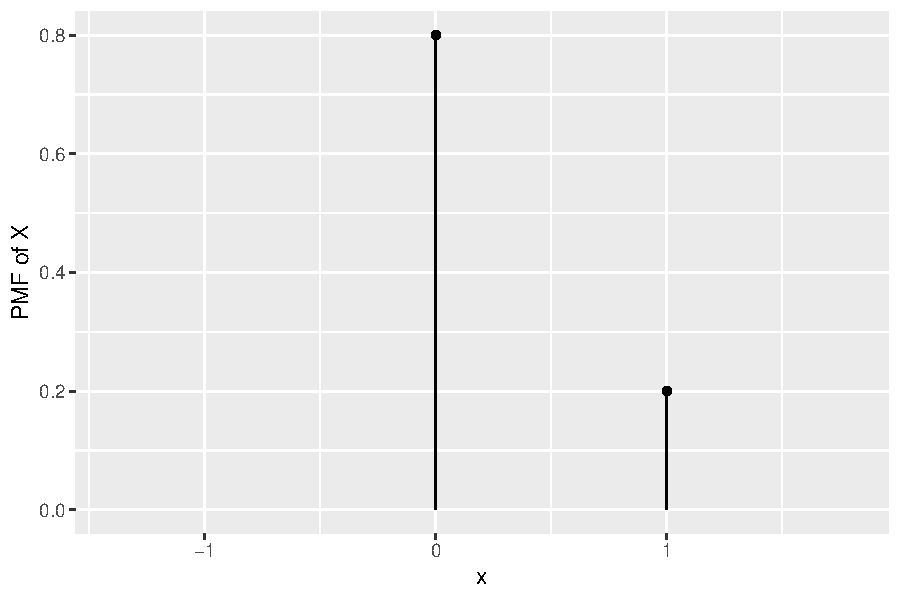
\includegraphics[width = .5\textwidth]{figure/clt1c-1} &
      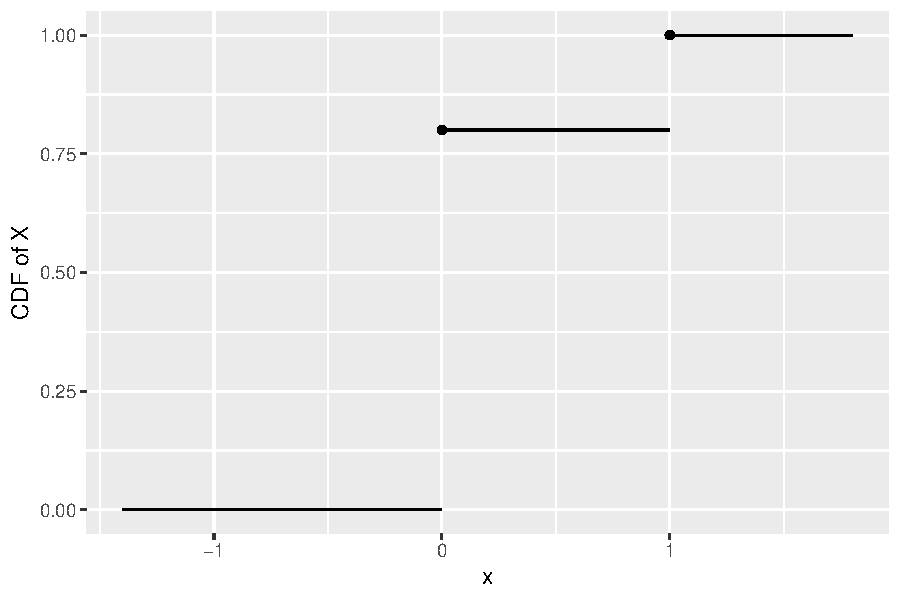
\includegraphics[width = .5\textwidth]{figure/clt1c-2}
      \end{tabular}
  
  \end{center}
\end{frame}

\begin{frame}
  
  \begin{center}
    \only<1>{
      PMF \& CDF of $Z=\frac{\sqrt{n}\left(\bar X_n - p \right)}{\sqrt{p(1-p)}}$ when $p=0.2$ and $n=2$
  
      \begin{tabular}{cc}
      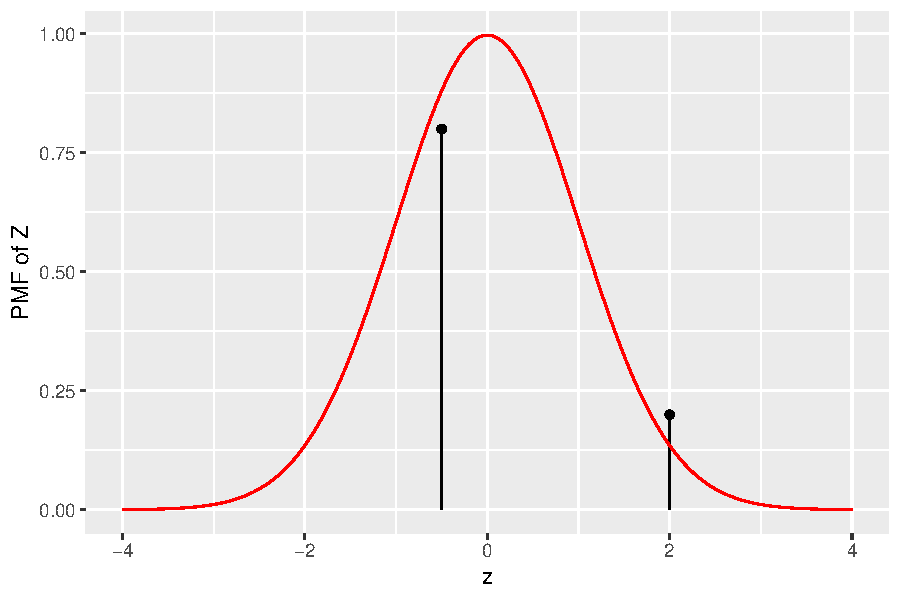
\includegraphics[width = .5\textwidth]{figure/clt1-1} &
      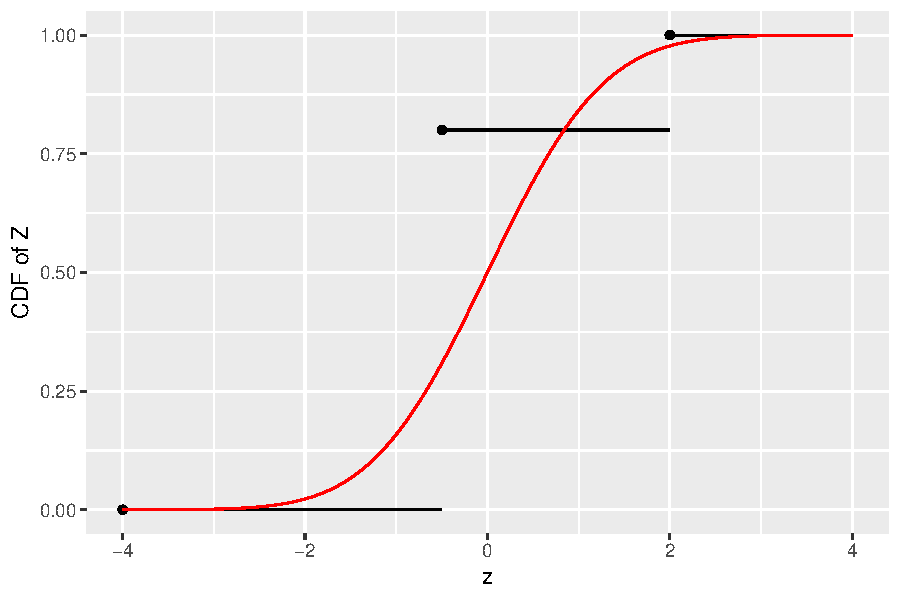
\includegraphics[width = .5\textwidth]{figure/clt1-2}
      \end{tabular}
    }
    \only<2>{
      PMF \& CDF of $Z=\frac{\sqrt{n}\left(\bar X_n - p \right)}{\sqrt{p(1-p)}}$ when $p=0.2$ and $n=5$
  
      \begin{tabular}{cc}
      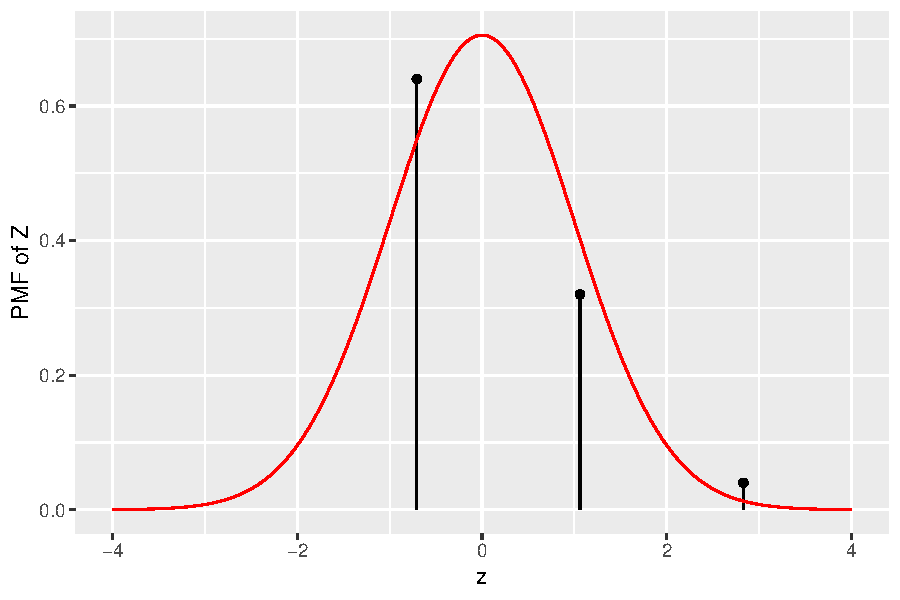
\includegraphics[width = .5\textwidth]{figure/clt1-3} &
      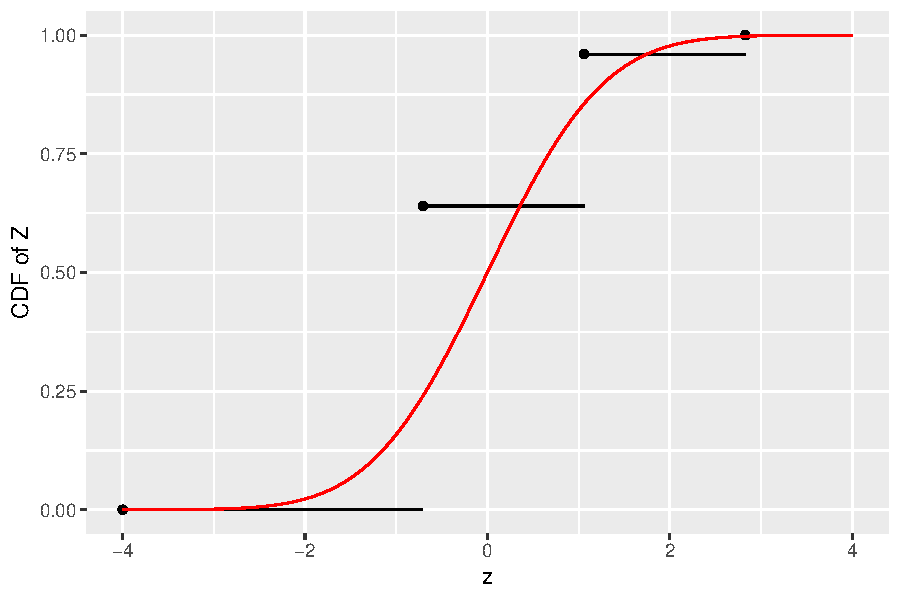
\includegraphics[width = .5\textwidth]{figure/clt1-4}
      \end{tabular}
    }
    \only<3>{
      PMF \& CDF of $Z=\frac{\sqrt{n}\left(\bar X_n - p \right)}{\sqrt{p(1-p)}}$ when $p=0.2$ and $n=10$
  
      \begin{tabular}{cc}
      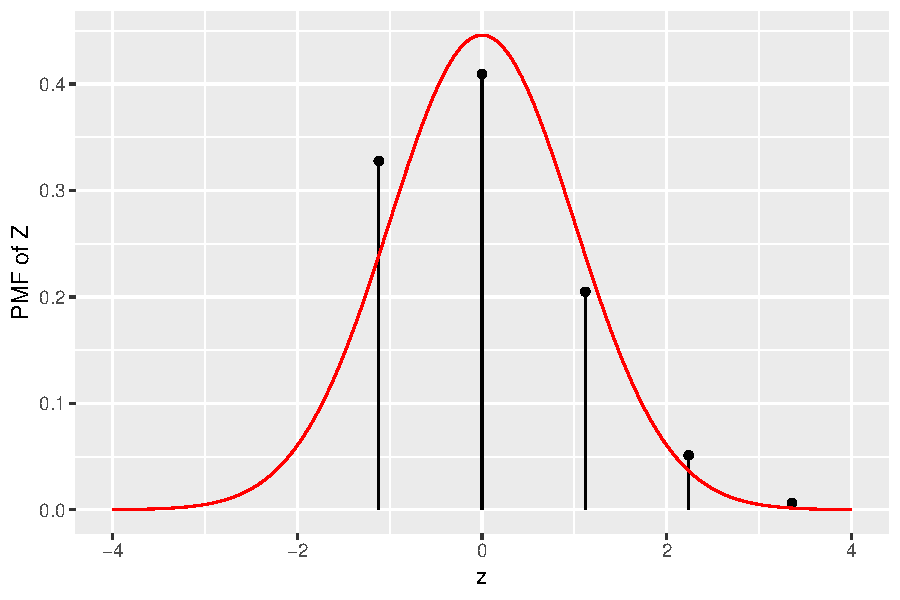
\includegraphics[width = .5\textwidth]{figure/clt1-5} &
      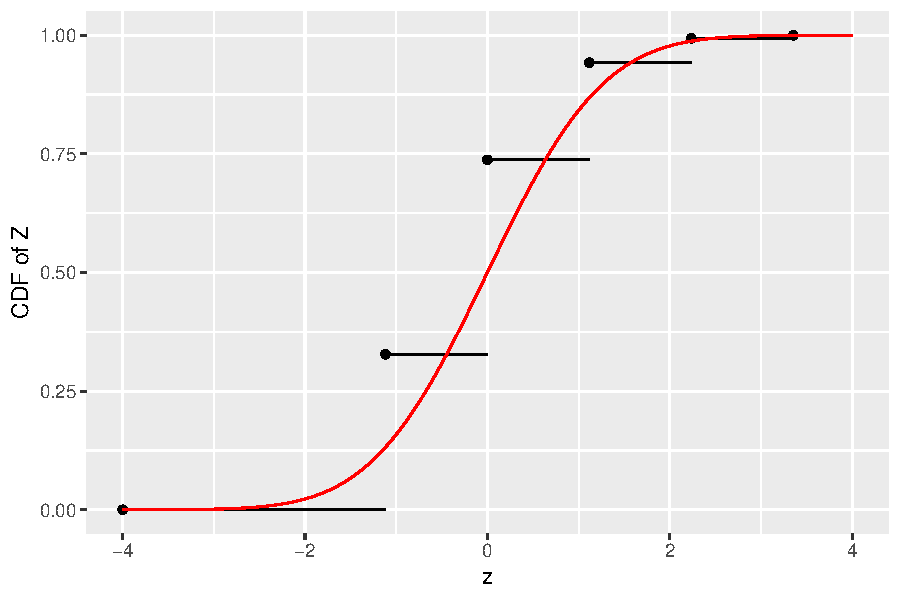
\includegraphics[width = .5\textwidth]{figure/clt1-6}
      \end{tabular}
    }
    \only<4>{
      PMF \& CDF of $Z=\frac{\sqrt{n}\left(\bar X_n - p \right)}{\sqrt{p(1-p)}}$ when $p=0.2$ and $n=25$
  
      \begin{tabular}{cc}
      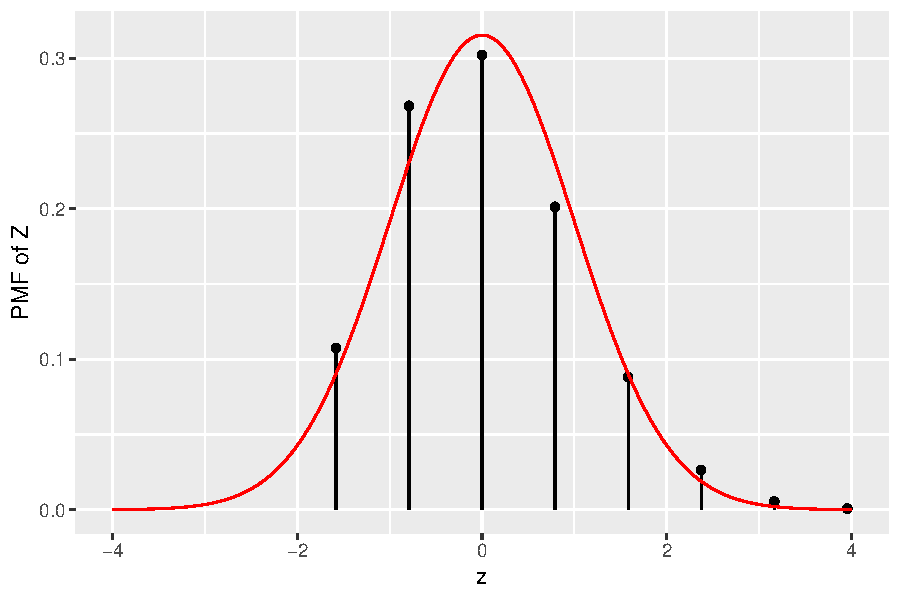
\includegraphics[width = .5\textwidth]{figure/clt1-7} &
      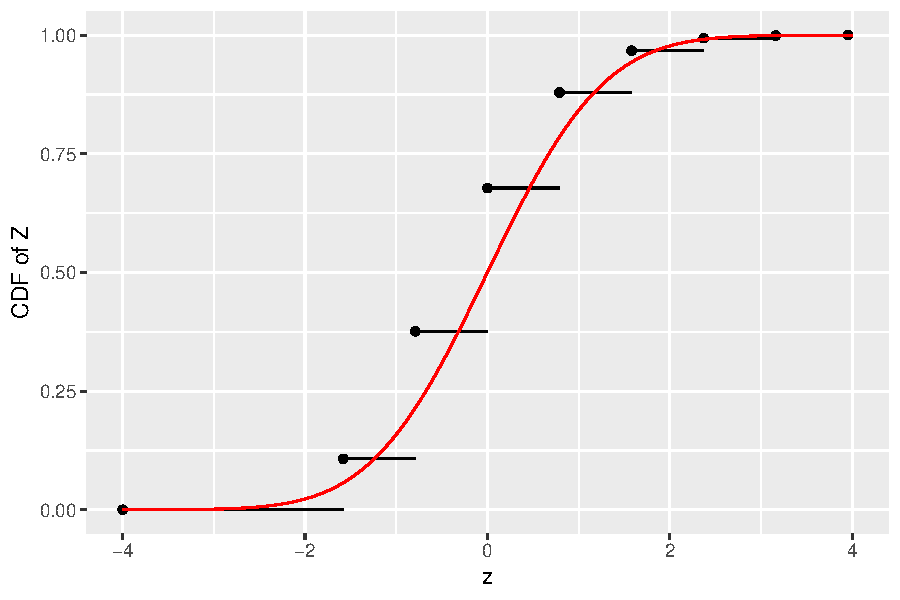
\includegraphics[width = .5\textwidth]{figure/clt1-8}
      \end{tabular}
    }
    \only<5>{
      PMF \& CDF of $Z=\frac{\sqrt{n}\left(\bar X_n - p \right)}{\sqrt{p(1-p)}}$ when $p=0.2$ and $n=50$
  
      \begin{tabular}{cc}
      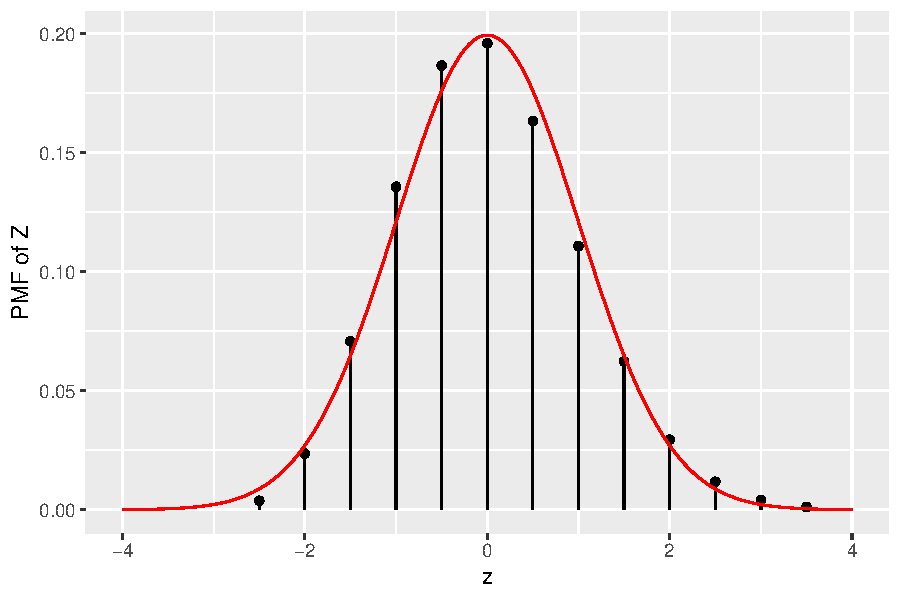
\includegraphics[width = .5\textwidth]{figure/clt1-9} &
      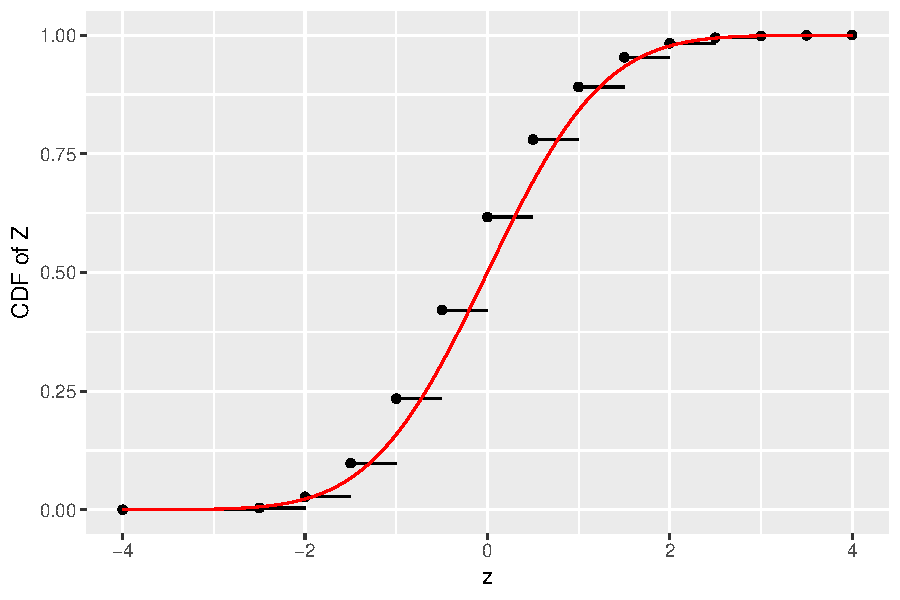
\includegraphics[width = .5\textwidth]{figure/clt1-10}
      \end{tabular}
    }
    \only<6>{
      PMF \& CDF of $Z=\frac{\sqrt{n}\left(\bar X_n - p \right)}{\sqrt{p(1-p)}}$ when $p=0.2$ and $n=100$
  
      \begin{tabular}{cc}
      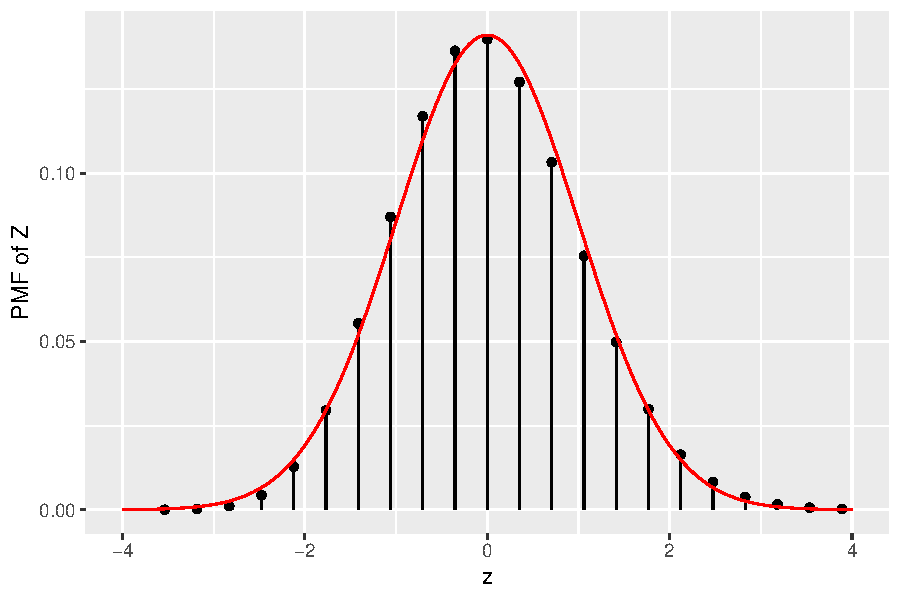
\includegraphics[width = .5\textwidth]{figure/clt1-11} &
      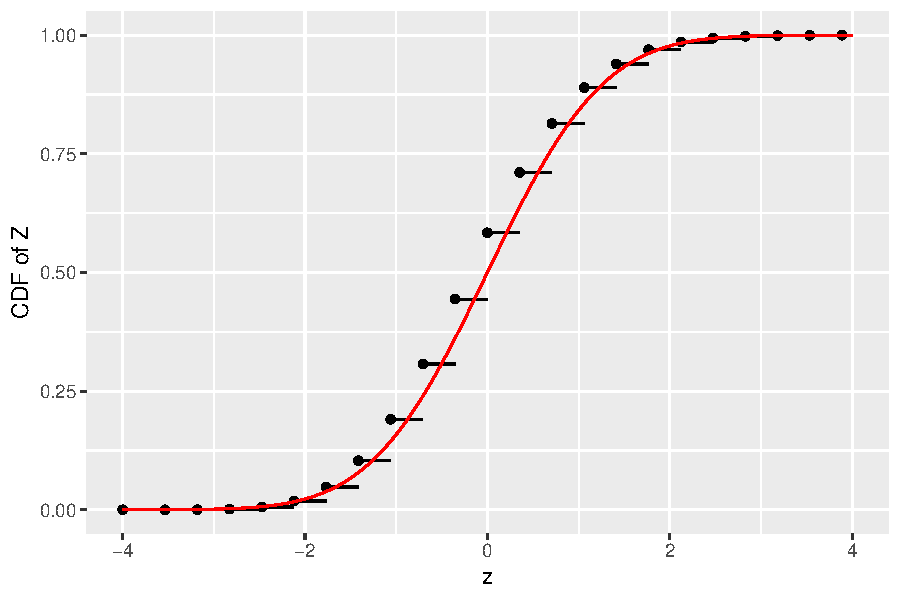
\includegraphics[width = .5\textwidth]{figure/clt1-12}
      \end{tabular}
    }
    \only<7>{
      PMF \& CDF of $Z=\frac{\sqrt{n}\left(\bar X_n - p \right)}{\sqrt{p(1-p)}}$ when $p=0.2$ and $n=100$
  
      \begin{tabular}{cc}
      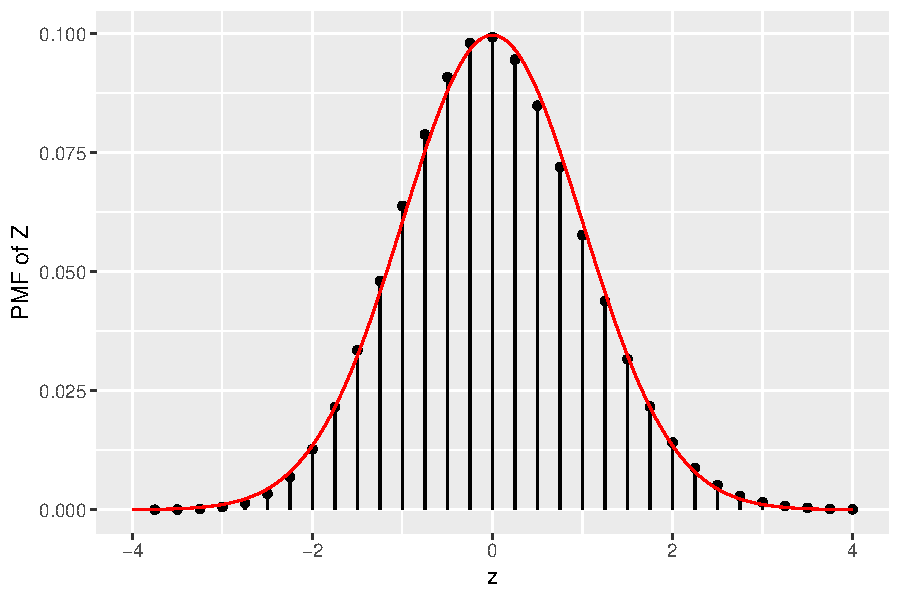
\includegraphics[width = .5\textwidth]{figure/clt1-13} &
      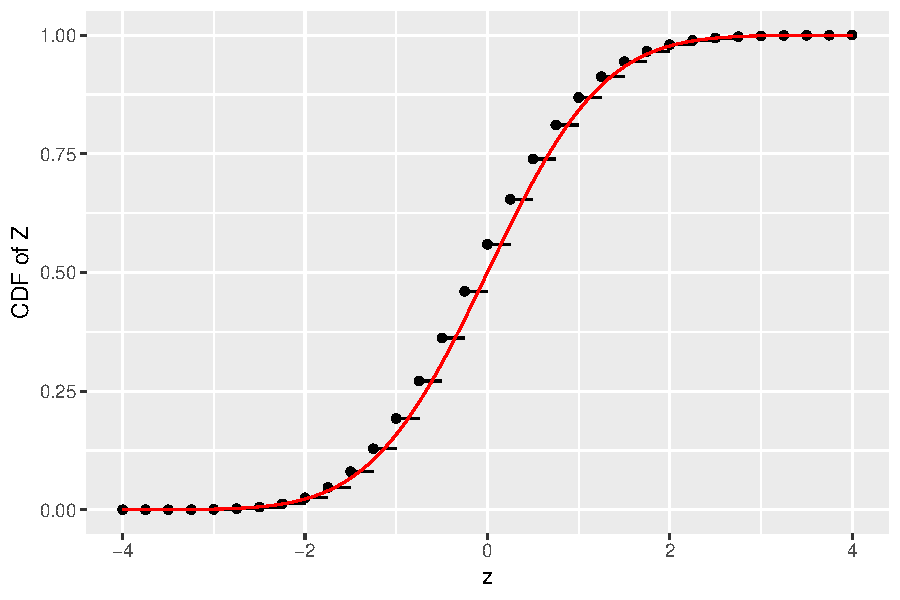
\includegraphics[width = .5\textwidth]{figure/clt1-14}
      \end{tabular}
    }
  \end{center}
  
\end{frame}

% <<clt2>>=

% n <- c(2,5,10,25,50,100,1000)

% p <- .1

% for(ni in n){
    
%     mydf <- tibble(x=(0:ni)/ni,
%                    zero=rep(0,ni+1),
%                    p=dbinom(0:ni,ni,p))
    
%     myplot <- ggplot(mydf,aes(x=x,y=p)) +
%         geom_point() + 
%         geom_segment(aes(x=x,xend=x,y=zero,yend=p)) + 
%         ylab("CDF of Sample Mean")
    
%     print(myplot)
    
% }

% @ 

% \begin{frame}
  
%   \begin{center}
%     \only<1>{
%       CDF of the Sample Mean when $p=.1$ and $n=2$
  
%       \includegraphics[height = .75\textheight]{figure/clt2-1}
%     }
%     \only<2>{
%       CDF of the Sample Mean when $p=.1$ and $n=5$
  
%       \includegraphics[height = .75\textheight]{figure/clt2-2}
%     }
%     \only<3>{
%       CDF of the Sample Mean when $p=.1$ and $n=10$
  
%       \includegraphics[height = .75\textheight]{figure/clt2-3}
%     }
%     \only<4>{
%       CDF of the Sample Mean when $p=.1$ and $n=25$
  
%       \includegraphics[height = .75\textheight]{figure/clt2-4}
%     }
%     \only<5>{
%       CDF of the Sample Mean when $p=.1$ and $n=50$
  
%       \includegraphics[height = .75\textheight]{figure/clt2-5}
%     }
%     \only<6>{
%       CDF of the Sample Mean when $p=.1$ and $n=100$
  
%       \includegraphics[height = .75\textheight]{figure/clt2-6}
%     }
%     %% \only<7>{
%     %%   CDF of the Sample Mean when $p=.1$ and $n=1000$
  
%     %%   \includegraphics[height = .75\textheight]{figure/clt2-7}
%     %% }
%   \end{center}
  
% \end{frame}



\begin{frame}
  \begin{block}{\example}
    Consider the random variable $Y$ with pmf
    \begin{center}
% latex table generated in R 4.4.1 by xtable 1.8-4 package
% Wed Nov 27 10:52:21 2024
\begin{table}[ht]
\centering
\begin{tabular}{rlllll}
  \hline
  \hline
y & 31 & 35 & 59 & 60 & 67 \\ 
  p & 0.24 & 0.15 & 0.23 & 0.32 & 0.06 \\ 
   \hline
\end{tabular}
\end{table}


    \end{center}
  \end{block}

  The mean and variance of $Y$ are
  \[
    \mu = E(Y)=49.45 \mbox{ and } \sigma^2=V(Y)=189.13.
  \]

\end{frame}



\begin{frame}

  \begin{center}
    PMF \& CDF of $Y$
    
      \begin{tabular}{cc}
      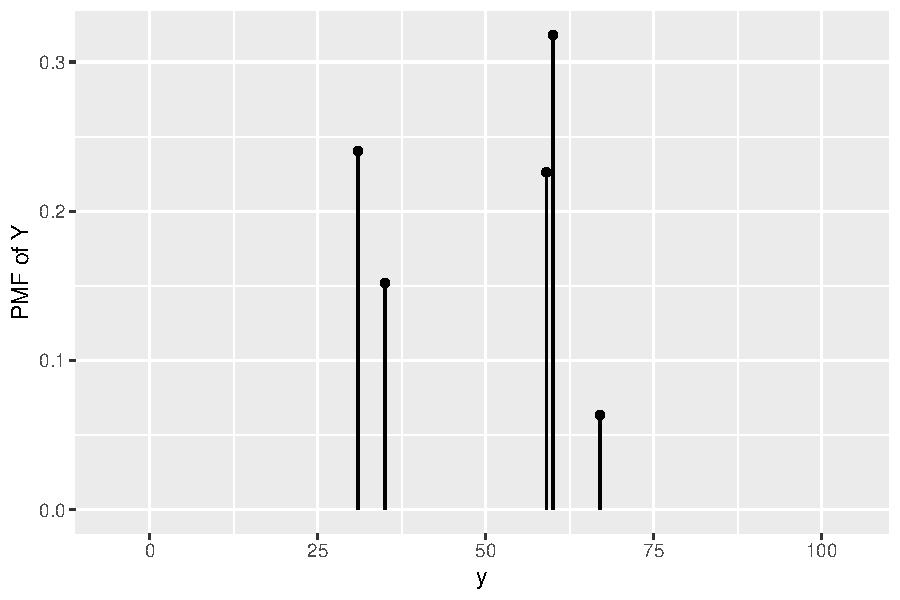
\includegraphics[width = .5\textwidth]{figure/clt3c-1} &
      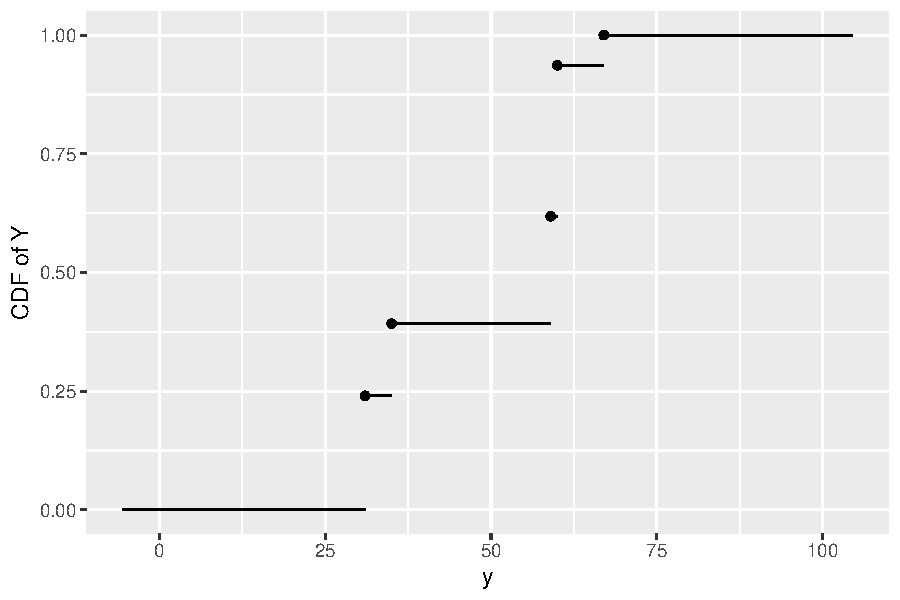
\includegraphics[width = .5\textwidth]{figure/clt3c-2}
      \end{tabular}
  
  \end{center}
\end{frame}

\begin{frame}
  
  \begin{center}
    \only<1>{
      PMF \& CDF of $Z=\frac{\sqrt{n}\left(\bar Y_n - \mu \right)}{\sigma}$ when $n=1$
  
      \begin{tabular}{cc}
      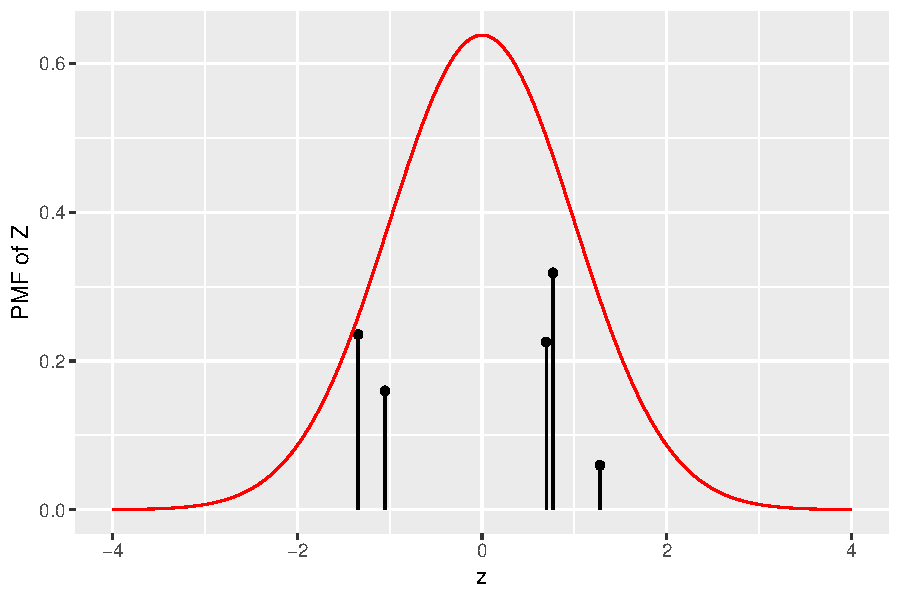
\includegraphics[width = .5\textwidth]{figure/clt3-1} &
      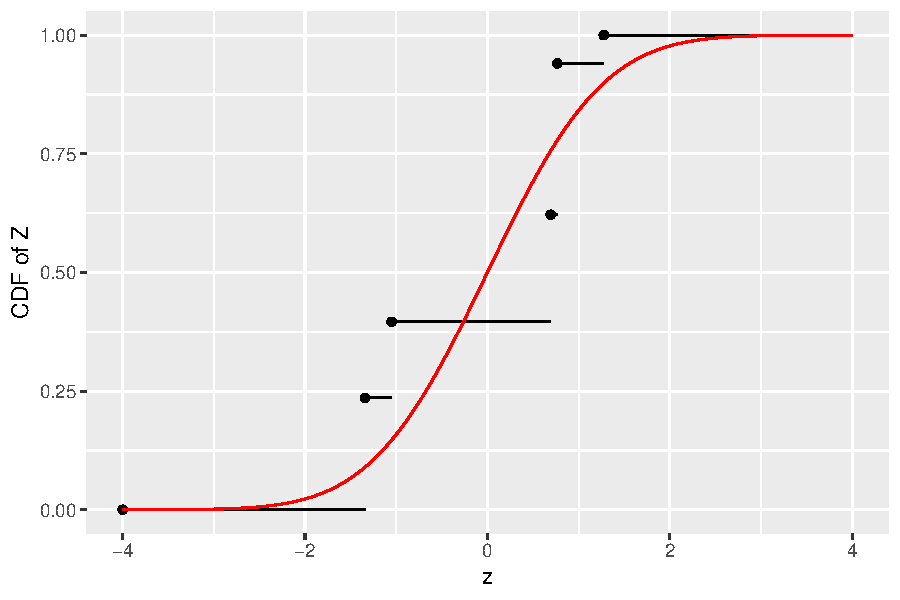
\includegraphics[width = .5\textwidth]{figure/clt3-2}
      \end{tabular}
     }
    \only<2>{
      PMF \& CDF of $Z=\frac{\sqrt{n}\left(\bar Y_n - \mu \right)}{\sigma}$ when $n=2$
  
      \begin{tabular}{cc}
      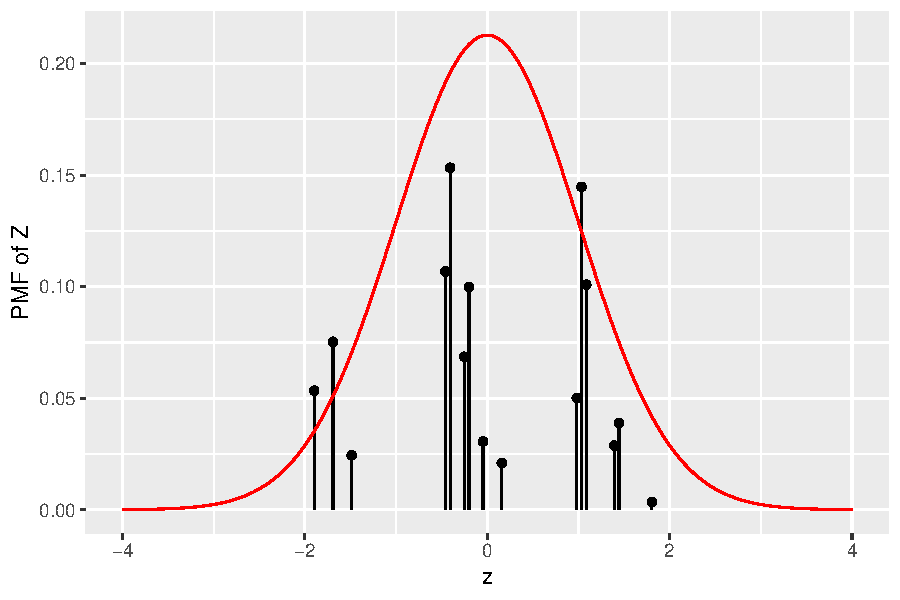
\includegraphics[width = .5\textwidth]{figure/clt3-3} &
      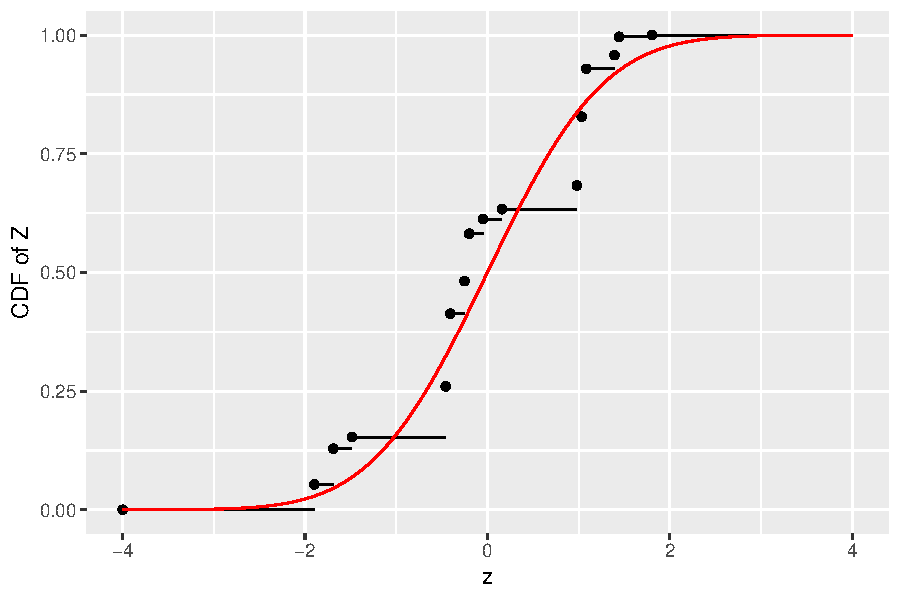
\includegraphics[width = .5\textwidth]{figure/clt3-4}
      \end{tabular}
     }
    \only<3>{
      PMF \& CDF of $Z=\frac{\sqrt{n}\left(\bar Y_n - \mu \right)}{\sigma}$ when $n=5$
  
      \begin{tabular}{cc}
      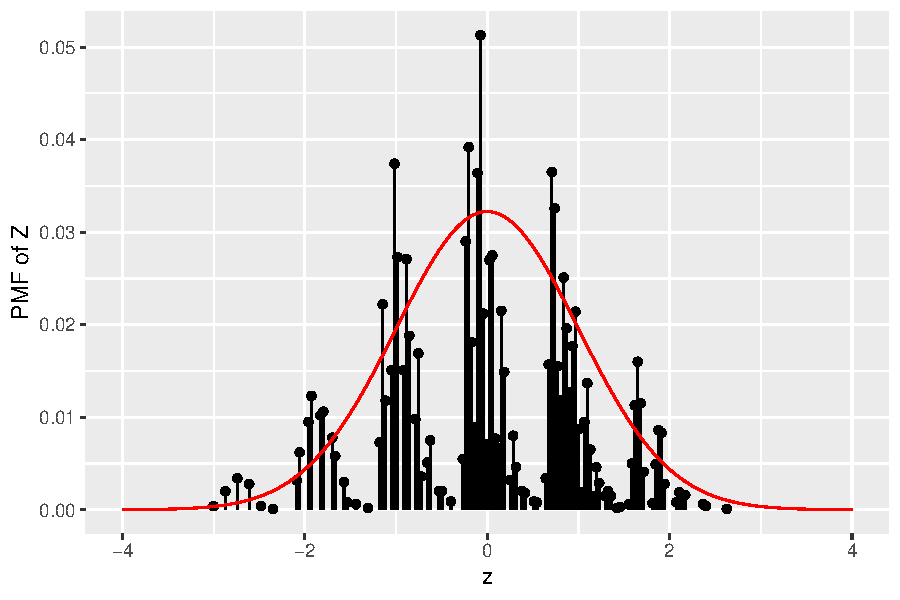
\includegraphics[width = .5\textwidth]{figure/clt3-5} &
      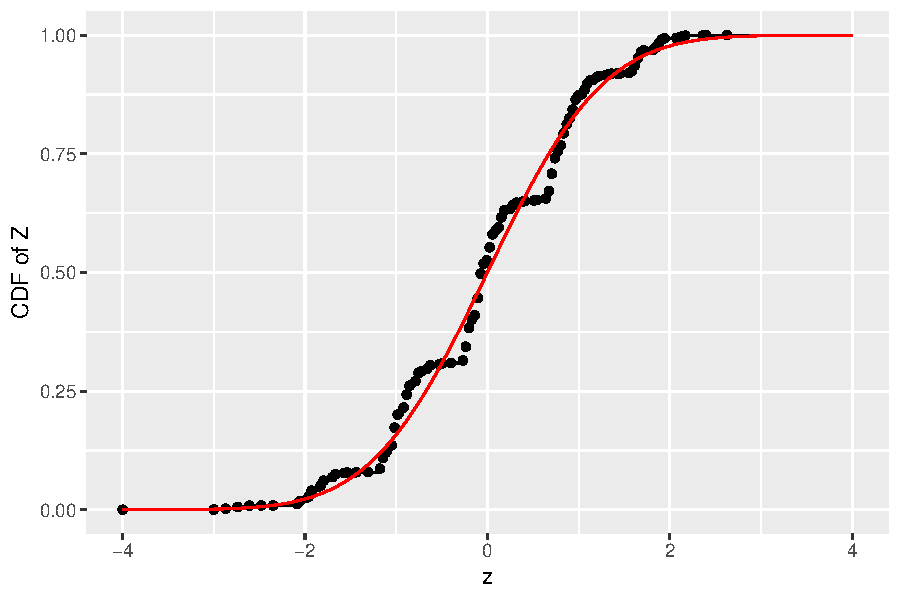
\includegraphics[width = .5\textwidth]{figure/clt3-6}
      \end{tabular}
     }
    \only<4>{
      PMF \& CDF of $Z=\frac{\sqrt{n}\left(\bar Y_n - \mu \right)}{\sigma}$ when $n=10$
  
      \begin{tabular}{cc}
      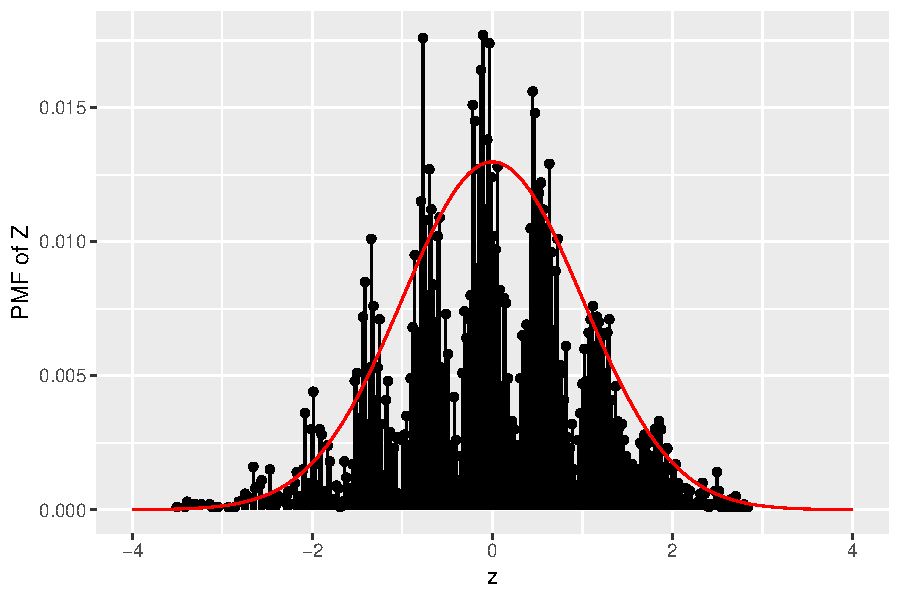
\includegraphics[width = .5\textwidth]{figure/clt3-7} &
      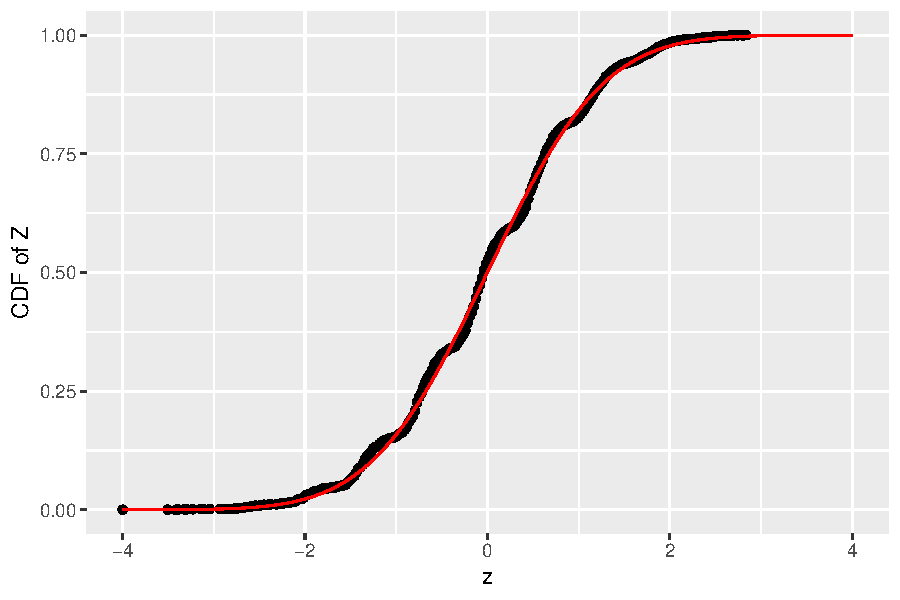
\includegraphics[width = .5\textwidth]{figure/clt3-8}
      \end{tabular}
     }
    \only<5>{
      PMF \& CDF of $Z=\frac{\sqrt{n}\left(\bar Y_n - \mu \right)}{\sigma}$ when $n=25$
  
      \begin{tabular}{cc}
      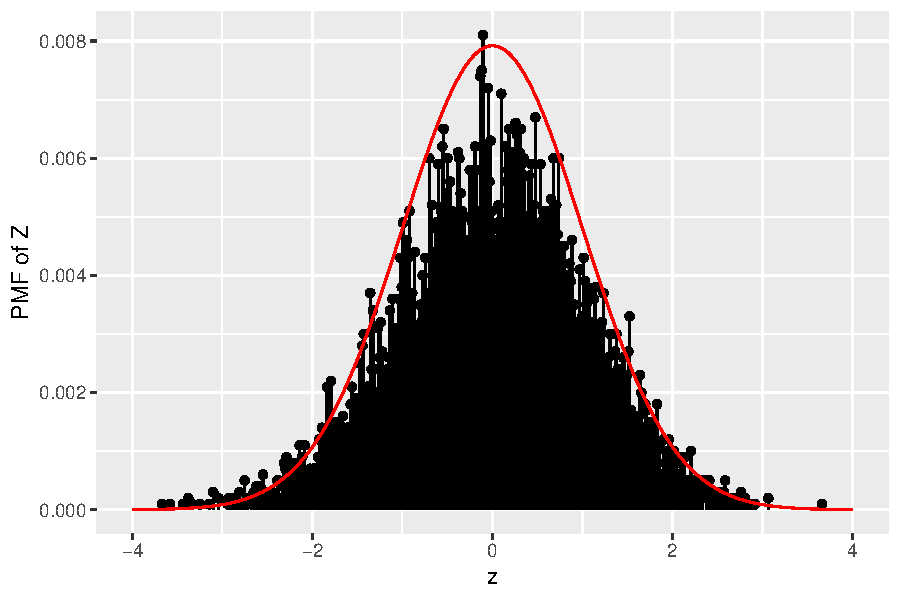
\includegraphics[width = .5\textwidth]{figure/clt3-9} &
      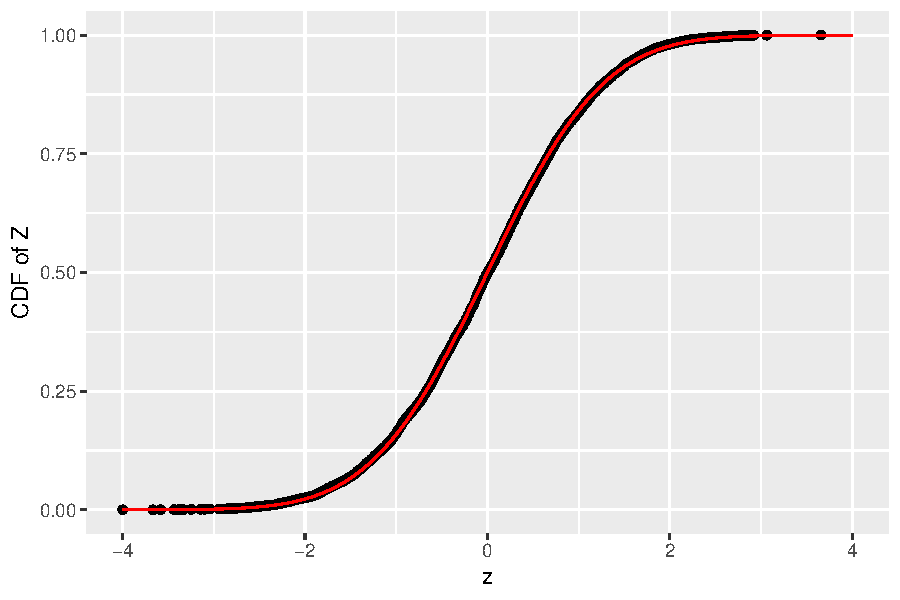
\includegraphics[width = .5\textwidth]{figure/clt3-10}
      \end{tabular}
     }
    \only<6>{
      PMF \& CDF of $Z=\frac{\sqrt{n}\left(\bar Y_n - \mu \right)}{\sigma}$ when $n=50$
  
      \begin{tabular}{cc}
      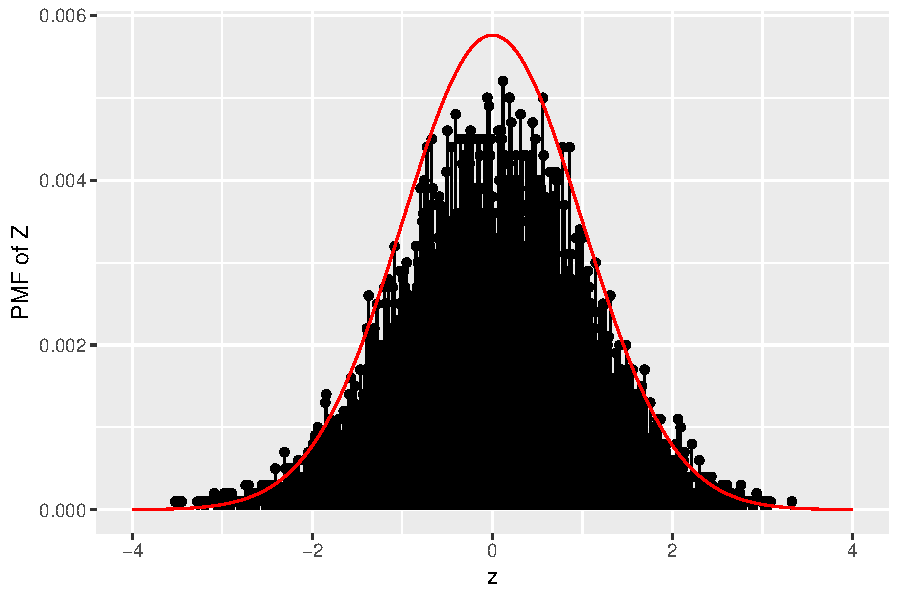
\includegraphics[width = .5\textwidth]{figure/clt3-11} &
      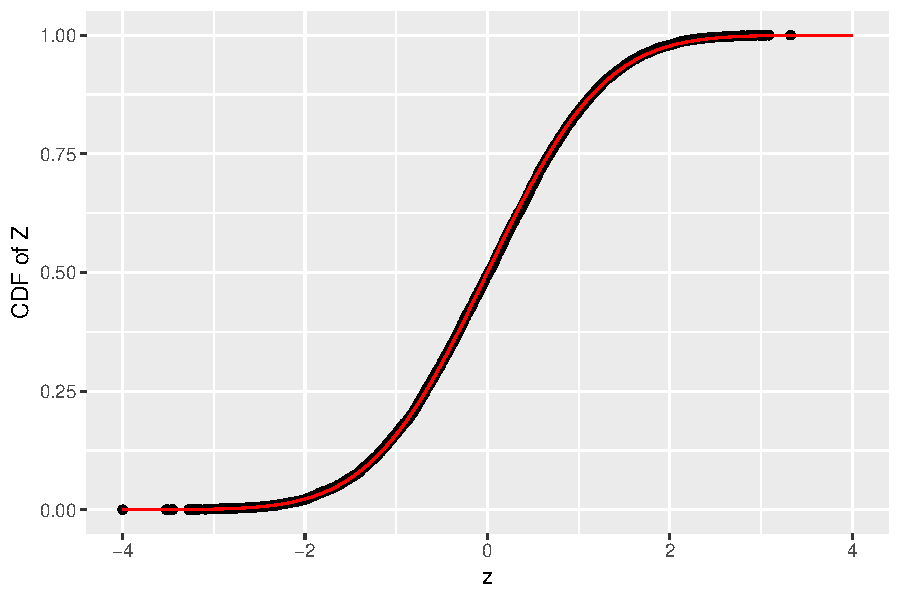
\includegraphics[width = .5\textwidth]{figure/clt3-12}
      \end{tabular}
     }
    \only<7>{
      PMF \& CDF of $Z=\frac{\sqrt{n}\left(\bar Y_n - \mu \right)}{\sigma}$ when $n=100$
  
      \begin{tabular}{cc}
      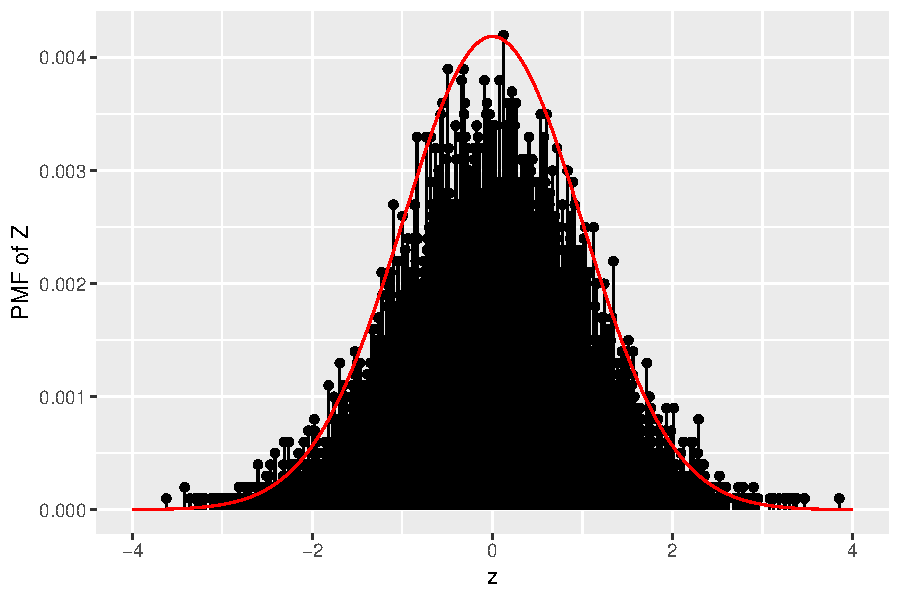
\includegraphics[width = .5\textwidth]{figure/clt3-13} &
      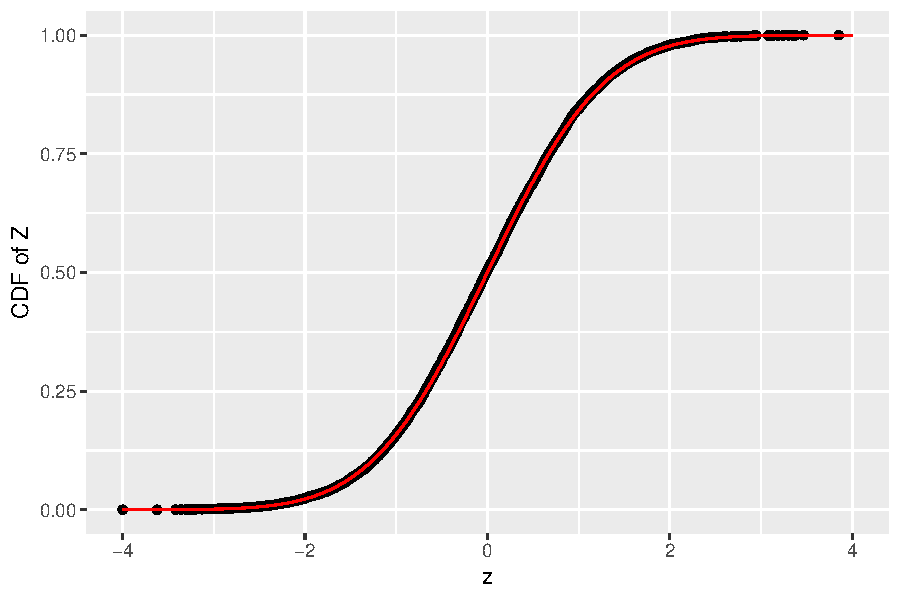
\includegraphics[width = .5\textwidth]{figure/clt3-14}
      \end{tabular}
     }
    %% \only<7>{
    %%   PMF \& CDF of the Sample Mean when $n=1000$
  
    %%   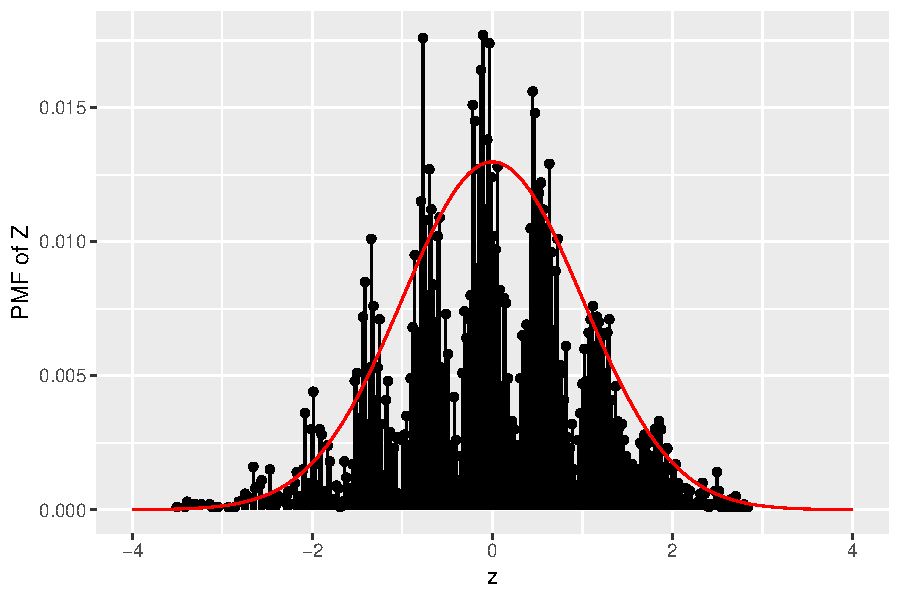
\includegraphics[height = .75\textheight]{figure/clt3-7}
    %% }
  \end{center}
  
\end{frame}


\begin{frame}
  \begin{block}{\example}
    The Acme string company produces spools of string advertised to have a length of 100~m. However, the length of string on a randomly selected ball actually has a mean of 101~m and a standard deviation of .2~m.

    \bigskip
    
    Approximate the 95-th percentile of the total amount of string in a box containing 50 spools.
  \end{block}
\end{frame}

\begin{frame}

  \begin{center}
    \Large{\textbf{Questions?}}
  \end{center}
\end{frame}

\begin{frame}

  \begin{block}{\exercise}
  According to Burmaster and Murray (1998), the log weight in kilograms of men between the ages of 50 and 80 is normally distributed with a mean of $4.41$ and variance $.46$. It can be shown that the weight then follows a log-normal distribution with mean $\mu_W = 91.45$~kg and variance $\sigma^2_W$1970.83~kg. The pdf is shown on the next slide. The vertical dashed line represents the mean.
  
  Let $W_1,\ldots,W_n$ be a random sample of weights for $n$ men.
  
  \begin{enumerate}[a)]
  \item Describe the shape of the density.
  \item Approximate the distribution of $\bar W_n$. What conditions need to be satisfied?
  \item Explain what the approximation in the previous part means.
  \item (Extra) Use the approximation to show that $\lim_{n \to \infty} P(\mu_W-\epsilon < \bar W_n < \mu_W + \epsilon) = 1$ for any $\epsilon>0$. Explain what this means.  
  \end{enumerate}
  \end{block}
\end{frame}



\end{document}

